\documentclass[8pt,aspectratio=1610]{beamer}
\usepackage[utf8]{inputenc}
\usepackage{booktabs}
\usepackage{array}
\usepackage{graphicx}
\usepackage{xcolor}
\usepackage{tikz}
\usetikzlibrary{positioning}
\usepackage{pgfplots}
\pgfplotsset{compat=1.18}

\usetheme{metropolis}
\usecolortheme{wolverine}
\metroset{progressbar=frametitle,block=fill}
\setbeamertemplate{navigation symbols}{}

\title{Exploratory Data Analysis (EDA)}
\subtitle{CMSC 173 - Machine Learning}
\author{Course Lecture}
\date{}

\begin{document}

\begin{frame}
\titlepage
\end{frame}

\begin{frame}{What is Exploratory Data Analysis?}
\begin{columns}[t]
\begin{column}{0.48\textwidth}
\begin{block}{Definition}
\textbf{EDA} is the process of investigating datasets to summarize their main characteristics, often using statistical graphics and other data visualization methods.
\end{block}

\vspace{0.3cm}
\textbf{Primary Goals:}
\begin{itemize}
\setlength{\itemsep}{1pt}
\item \textcolor{blue}{\textbf{Understand}} data structure and quality
\item \textcolor{red}{\textbf{Discover}} patterns and relationships
\item \textcolor{green}{\textbf{Identify}} anomalies and outliers
\item \textcolor{orange}{\textbf{Guide}} feature engineering decisions
\item \textcolor{purple}{\textbf{Inform}} modeling strategy
\end{itemize}

\vspace{0.3cm}
\textbf{Key Questions EDA Answers:}
\begin{itemize}
\setlength{\itemsep}{1pt}
\item What does my data look like?
\item Is my data clean and complete?
\item What patterns exist?
\item Which features are important?
\end{itemize}
\end{column}

\begin{column}{0.48\textwidth}
\textbf{EDA Process Overview:}
\vspace{0.2cm}

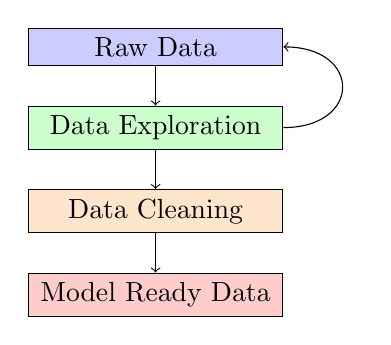
\begin{tikzpicture}[node distance=1cm]
\node[rectangle, draw, fill=blue!20, text width=3cm, text centered] (data) {Raw Data};
\node[rectangle, draw, fill=green!20, text width=3cm, text centered, below=0.5cm of data] (explore) {Data Exploration};
\node[rectangle, draw, fill=orange!20, text width=3cm, text centered, below=0.5cm of explore] (clean) {Data Cleaning};
\node[rectangle, draw, fill=red!20, text width=3cm, text centered, below=0.5cm of clean] (model) {Model Ready Data};

\draw[->] (data) -- (explore);
\draw[->] (explore) -- (clean);
\draw[->] (clean) -- (model);
\draw[->] (explore.east) .. controls +(right:1cm) and +(right:1cm) .. (data.east);
\end{tikzpicture}

\vspace{0.4cm}
\begin{alertblock}{Remember}
\textbf{EDA is iterative!} Insights from one analysis often lead to new questions and deeper investigations.
\end{alertblock}
\end{column}
\end{columns}
\end{frame}

\begin{frame}{Data Types in Tabular Data: Titanic Example}
\vspace{-0.3cm}

\begin{block}{Example: Titanic Survival Data Set}
Contains information on 1309 passengers aboard the Titanic and whether they survived or not. Goal: To predict the survival of passengers based on their attributes.
\end{block}

\vspace{0.2cm}
\textbf{For tabular data, different \underline{data types} can exist in one table.}

\vspace{0.3cm}
\begin{center}
\tiny
\begin{tabular}{|c|c|c|l|c|c|c|c|c|c|}
\hline
\textbf{ID} & \textbf{Survived} & \textbf{Pclass} & \textbf{Name} & \textbf{Sex} & \textbf{Age} & \textbf{SibSp} & \textbf{Parch} & \textbf{Fare} & \textbf{Embarked} \\
\hline
0 & 1 & 3 & Braund, Mr. Owen Harris & male & 22.0 & 1 & 0 & 7.25 & S \\
\hline
1 & 1 & 1 & Cumings, Mrs. John Bradley & female & 38.0 & 1 & 0 & 71.28 & C \\
\hline
2 & 1 & 3 & Heikkinen, Miss. Laina & female & 26.0 & 0 & 0 & 7.92 & S \\
\hline
3 & 1 & 1 & Futrelle, Mrs. Jacques Heath & female & 35.0 & 1 & 0 & 53.10 & S \\
\hline
4 & 0 & 3 & Allen, Mr. William Henry & male & 35.0 & 0 & 0 & 8.05 & S \\
\hline
\end{tabular}
\end{center}

\vspace{0.2cm}
% Data type arrows and labels using text positioning instead of overlay
\begin{center}
\scriptsize
\textcolor{blue}{Integer,} \hspace{0.5cm} \textcolor{red}{Integer,} \hspace{0.5cm} \textcolor{purple}{Integer,} \hspace{1.5cm} \textcolor{green}{String} \hspace{0.5cm} \textcolor{orange}{String,} \hspace{0.5cm} \textcolor{cyan}{Continuous} \hspace{0.2cm} \textcolor{magenta}{Integer,} \hspace{0.2cm} \textcolor{brown}{Integer,} \hspace{0.2cm} \textcolor{gray}{Continuous} \hspace{0.2cm} \textcolor{teal}{String,} \\
\textcolor{blue}{Ordinal} \hspace{0.7cm} \textcolor{red}{Binary} \hspace{0.7cm} \textcolor{purple}{Categorical} \hspace{0.5cm} \hspace{1.5cm} \textcolor{orange}{Categorical} \hspace{1.2cm} \textcolor{magenta}{Non-negative} \hspace{0.2cm} \textcolor{brown}{Non-negative} \hspace{1.0cm} \textcolor{teal}{Categorical}
\end{center}

\vspace{1.0cm}
\begin{columns}
\begin{column}{0.48\textwidth}
\textbf{Attributes:}
\begin{itemize}
\setlength{\itemsep}{2pt}
\item \textcolor{red}{\textbf{Passenger ID}} - An identifier unique to a passenger
\item \textcolor{red}{\textbf{Survived}} - 1 = survived, 0 = did not survive
\item \textcolor{red}{\textbf{Pclass}} - 1, 2, 3 = travel class
\item \textcolor{red}{\textbf{Name}} - Passenger's name
\item \textcolor{red}{\textbf{Sex}} - Male / Female
\end{itemize}
\end{column}

\begin{column}{0.48\textwidth}
\begin{itemize}
\setlength{\itemsep}{2pt}
\item \textcolor{red}{\textbf{Age}} - Passenger's age
\item \textcolor{red}{\textbf{SibSp}} - Number of siblings and spouses aboard
\item \textcolor{red}{\textbf{Parch}} - Number of parents and children aboard
\item \textcolor{red}{\textbf{Ticket}} - Ticket number
\item \textcolor{red}{\textbf{Fare}} - Amount paid for ticket
\item \textcolor{red}{\textbf{Cabin}} - Cabin of residence
\item \textcolor{red}{\textbf{Embarked}} - Q = Queenstown, C = Cherbourg, S = Southampton
\end{itemize}
\end{column}
\end{columns}
\end{frame}

\begin{frame}{Data Modalities and Types}
\begin{columns}[t]
\begin{column}{0.48\textwidth}
\textbf{Data Modalities:}
\begin{itemize}
\setlength{\itemsep}{1pt}
\item \textcolor{blue}{\textbf{Structured:}} Tables, CSV, databases
\item \textcolor{red}{\textbf{Semi-structured:}} JSON, XML, logs
\item \textcolor{green}{\textbf{Unstructured:}} Text, images, audio, video
\end{itemize}

\vspace{0.3cm}
\begin{block}{Structured Data Example}
\scriptsize
\begin{tabular}{|c|c|c|c|}
\hline
\textbf{ID} & \textbf{Name} & \textbf{Age} & \textbf{Salary} \\
\hline
1 & Alice & 25 & 50000 \\
2 & Bob & 30 & 65000 \\
3 & Carol & 28 & 58000 \\
\hline
\end{tabular}
\end{block}

\vspace{0.3cm}
\textbf{Data Attributes by Nature:}
\begin{itemize}
\setlength{\itemsep}{1pt}
\item \textbf{Quantitative:} Numerical measurements
\item \textbf{Qualitative:} Categorical descriptions
\end{itemize}
\end{column}

\begin{column}{0.48\textwidth}
\textbf{Detailed Data Types:}
\vspace{0.2cm}

\begin{block}{Numerical (Quantitative)}
\begin{itemize}
\setlength{\itemsep}{1pt}
\item \textcolor{blue}{\textbf{Continuous:}} Height, weight, temperature
\item \textcolor{red}{\textbf{Discrete:}} Count of items, number of children
\end{itemize}
\end{block}

\begin{block}{Categorical (Qualitative)}
\begin{itemize}
\setlength{\itemsep}{1pt}
\item \textcolor{green}{\textbf{Nominal:}} Colors, gender, country
\item \textcolor{orange}{\textbf{Ordinal:}} Grade (A,B,C), satisfaction levels
\item \textcolor{purple}{\textbf{Binary:}} Yes/No, True/False
\end{itemize}
\end{block}

\textbf{Special Types:}
\begin{itemize}
\setlength{\itemsep}{1pt}
\item \textbf{DateTime:} Timestamps, dates
\item \textbf{Text:} Free-form text, descriptions
\item \textbf{Geospatial:} Coordinates, addresses
\item \textbf{Mixed:} Combinations of above types
\end{itemize}
\end{column}
\end{columns}
\end{frame}

\begin{frame}{Data Understanding: First Look}
\begin{columns}[t]
\begin{column}{0.48\textwidth}
\textbf{Initial Data Exploration:}
\begin{itemize}
\setlength{\itemsep}{1pt}
\item \texttt{df.shape} - Dimensions (rows, columns)
\item \texttt{df.info()} - Data types and memory usage
\item \texttt{df.head()}, \texttt{df.tail()} - Sample records
\item \texttt{df.describe()} - Summary statistics
\item \texttt{df.columns} - Column names
\end{itemize}

\vspace{0.3cm}
\begin{exampleblock}{Titanic Dataset Example}
\scriptsize
\texttt{df.shape: (891, 12)} \\
\texttt{df.info(): 714 non-null Age, 891 non-null Sex} \\
\texttt{Target: Survived (binary)}
\end{exampleblock}
\end{column}

\begin{column}{0.48\textwidth}
\textbf{Quick Visual Overview:}
\vspace{0.2cm}

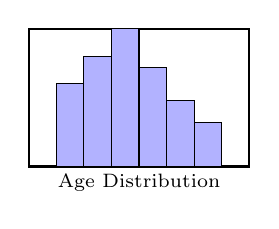
\begin{tikzpicture}[scale=0.7]
% Histogram placeholder
\draw[thick] (0,0) rectangle (4,2.5);
\draw[fill=blue!30] (0.5,0) rectangle (1,1.5);
\draw[fill=blue!30] (1,0) rectangle (1.5,2);
\draw[fill=blue!30] (1.5,0) rectangle (2,2.5);
\draw[fill=blue!30] (2,0) rectangle (2.5,1.8);
\draw[fill=blue!30] (2.5,0) rectangle (3,1.2);
\draw[fill=blue!30] (3,0) rectangle (3.5,0.8);
\node at (2,-0.3) {\scriptsize Age Distribution};
\end{tikzpicture}

\vspace{0.3cm}
\textbf{Key Insights from First Look:}
\begin{itemize}
\setlength{\itemsep}{1pt}
\item \textcolor{red}{\textbf{Missing Data:}} Age has 177 missing values
\item \textcolor{blue}{\textbf{Data Types:}} Mix of numerical and categorical
\item \textcolor{green}{\textbf{Target Variable:}} Survived (binary classification)
\item \textcolor{orange}{\textbf{Features:}} 11 potential predictors
\end{itemize}
\end{column}
\end{columns}
\end{frame}

\begin{frame}{Handling Missing Values: Strategies}
\begin{columns}[t]
\begin{column}{0.5\textwidth}
\textbf{Missing Data Patterns:}
\begin{itemize}
\setlength{\itemsep}{1pt}
\item \textbf{MCAR:} Missing Completely At Random
\item \textbf{MAR:} Missing At Random
\item \textbf{MNAR:} Missing Not At Random
\end{itemize}

\vspace{0.3cm}
\textbf{Detection Methods:}
\begin{itemize}
\setlength{\itemsep}{1pt}
\item \texttt{df.isnull().sum()}
\item \texttt{df.info()}
\item Heatmaps: \texttt{sns.heatmap(df.isnull())}
\item Missing patterns visualization
\end{itemize}

\vspace{0.3cm}
\textbf{Handling Strategies:}
\begin{itemize}
\setlength{\itemsep}{1pt}
\item \textcolor{red}{Delete:} Listwise/Pairwise deletion
\item \textcolor{blue}{Impute:} Mean, median, mode, KNN
\item \textcolor{green}{Model:} Regression, ML-based imputation
\end{itemize}
\end{column}

\begin{column}{0.48\textwidth}
\textbf{Outlier Detection:}
\vspace{0.2cm}

\begin{block}{Statistical Methods}
\begin{itemize}
\setlength{\itemsep}{1pt}
\item \textbf{IQR Rule:} $Q_1 - 1.5 \times IQR$ to $Q_3 + 1.5 \times IQR$
\item \textbf{Z-score:} $|z| > 3$ (or 2.5)
\item \textbf{Modified Z-score:} Using median
\end{itemize}
\end{block}

\begin{block}{Visual Methods}
\begin{itemize}
\setlength{\itemsep}{1pt}
\item Box plots, violin plots
\item Scatter plots for bivariate
\item Histograms with overlays
\end{itemize}
\end{block}

\begin{block}{Advanced Methods}
\begin{itemize}
\setlength{\itemsep}{1pt}
\item Isolation Forest
\item Local Outlier Factor (LOF)
\item DBSCAN clustering
\end{itemize}
\end{block}
\end{column}
\end{columns}
\end{frame}

\begin{frame}{Column Transformations}
\begin{columns}[t]
\begin{column}{0.48\textwidth}
\textbf{Common Transformations:}
\begin{itemize}
\setlength{\itemsep}{1pt}
\item \textcolor{blue}{\textbf{Encoding:}} Convert categories to numbers
\item \textcolor{red}{\textbf{Scaling:}} Normalize numerical ranges
\item \textcolor{green}{\textbf{Binning:}} Group continuous values
\item \textcolor{orange}{\textbf{Feature Creation:}} Derive new features
\end{itemize}

\vspace{0.3cm}
\begin{block}{Categorical Encoding}
\textbf{One-Hot Encoding:}
\scriptsize
\begin{tabular}{|c|c|c|c|}
\hline
\textbf{Color} & \textbf{Red} & \textbf{Blue} & \textbf{Green} \\
\hline
Red & 1 & 0 & 0 \\
Blue & 0 & 1 & 0 \\
Green & 0 & 0 & 1 \\
\hline
\end{tabular}
\end{block}

\textbf{Label Encoding:}
\scriptsize
\begin{tabular}{|c|c|}
\hline
\textbf{Grade} & \textbf{Encoded} \\
\hline
A & 3 \\
B & 2 \\
C & 1 \\
F & 0 \\
\hline
\end{tabular}
\end{column}

\begin{column}{0.48\textwidth}
\textbf{Feature Engineering Examples:}
\vspace{0.2cm}

\begin{exampleblock}{From DateTime}
\scriptsize
\texttt{df['hour'] = df['timestamp'].dt.hour} \\
\texttt{df['is\_weekend'] = df['day\_of\_week'] > 4}
\end{exampleblock}

\begin{exampleblock}{From Text}
\scriptsize
\texttt{df['text\_length'] = df['review'].str.len()} \\
\texttt{df['has\_exclamation'] = df['review'].str.contains('!')}
\end{exampleblock}

\begin{exampleblock}{Mathematical Transformations}
\scriptsize
\texttt{df['log\_income'] = np.log1p(df['income'])} \\
\texttt{df['age\_income'] = df['age'] * df['income']}
\end{exampleblock}
\end{column}
\end{columns}
\end{frame}

\begin{frame}{Data Normalization and Scaling}
\begin{columns}[t]
\begin{column}{0.48\textwidth}
\textbf{Why Normalize?}
\begin{itemize}
\setlength{\itemsep}{1pt}
\item Different scales affect ML algorithms
\item Features with larger ranges dominate
\item Improves convergence speed
\item Required for distance-based algorithms
\end{itemize}

\vspace{0.3cm}
\begin{block}{Min-Max Scaling}
$$X_{scaled} = \frac{X - X_{min}}{X_{max} - X_{min}}$$
\textbf{Range:} [0, 1]
\textbf{Use:} When you know min/max bounds
\end{block}

\begin{block}{Z-Score Standardization}
$$X_{scaled} = \frac{X - \mu}{\sigma}$$
\textbf{Range:} $\mu = 0, \sigma = 1$
\textbf{Use:} When data is normally distributed
\end{block}
\end{column}

\begin{column}{0.48\textwidth}
\textbf{Scaling Methods Comparison:}
\vspace{0.2cm}

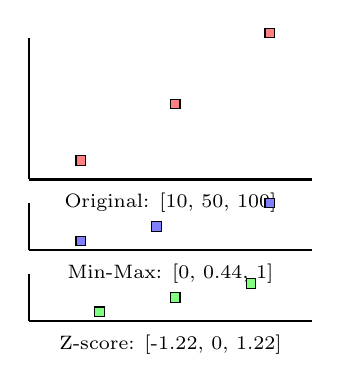
\begin{tikzpicture}[scale=0.6]
% Original data
\draw[thick] (0,0) -- (6,0);
\draw[thick] (0,0) -- (0,3);
\node at (3,-0.5) {\scriptsize Original: [10, 50, 100]};
\draw[fill=red!50] (1,0.3) rectangle (1.2,0.5);
\draw[fill=red!50] (3,1.5) rectangle (3.2,1.7);
\draw[fill=red!50] (5,3) rectangle (5.2,3.2);

% Min-Max scaled
\draw[thick] (0,-1.5) -- (6,-1.5);
\draw[thick] (0,-1.5) -- (0,-0.5);
\node at (3,-2) {\scriptsize Min-Max: [0, 0.44, 1]};
\draw[fill=blue!50] (1,-1.4) rectangle (1.2,-1.2);
\draw[fill=blue!50] (2.6,-1.1) rectangle (2.8,-0.9);
\draw[fill=blue!50] (5,-0.6) rectangle (5.2,-0.4);

% Z-score scaled
\draw[thick] (0,-3) -- (6,-3);
\draw[thick] (0,-3) -- (0,-2);
\node at (3,-3.5) {\scriptsize Z-score: [-1.22, 0, 1.22]};
\draw[fill=green!50] (1.4,-2.9) rectangle (1.6,-2.7);
\draw[fill=green!50] (3,-2.6) rectangle (3.2,-2.4);
\draw[fill=green!50] (4.6,-2.3) rectangle (4.8,-2.1);
\end{tikzpicture}

\vspace{0.3cm}
\begin{exampleblock}{Python Implementation}
\scriptsize
\texttt{scaler = MinMaxScaler()} \\
\texttt{X\_minmax = scaler.fit\_transform(X)} \\
\texttt{scaler = StandardScaler()} \\
\texttt{X\_standard = scaler.fit\_transform(X)}
\end{exampleblock}
\end{column}
\end{columns}
\end{frame}

\begin{frame}{Distribution Analysis and Visualization Examples}
\begin{columns}[t]
\begin{column}{0.48\textwidth}
\textbf{Numerical Variables:}
\begin{itemize}
\setlength{\itemsep}{1pt}
\item \textbf{Central Tendency:} Mean, median, mode
\item \textbf{Spread:} Variance, std dev, range, IQR
\item \textbf{Shape:} Skewness, kurtosis
\item \textbf{Normality Tests:} Shapiro-Wilk, Anderson-Darling
\end{itemize}

\vspace{0.3cm}
\begin{block}{Skewness Interpretation}
\begin{itemize}
\setlength{\itemsep}{1pt}
\item $-0.5 < $ Skew $ < 0.5$: Symmetric
\item $0.5 < |$Skew$| < 1$: Moderate
\item $|$Skew$| > 1$: Highly skewed
\end{itemize}
\end{block}

\textbf{Transformations:}
\begin{itemize}
\setlength{\itemsep}{1pt}
\item \textbf{Log:} Right-skewed data
\item \textbf{Square root:} Moderate skew
\item \textbf{Box-Cox:} Optimal transformation
\end{itemize}
\end{column}

\begin{column}{0.48\textwidth}
\textbf{Categorical Variables:}
\begin{itemize}
\setlength{\itemsep}{1pt}
\item \textbf{Frequency tables:} Value counts
\item \textbf{Proportions:} Relative frequencies
\item \textbf{Mode:} Most frequent category
\item \textbf{Cardinality:} Number of unique values
\end{itemize}

\vspace{0.3cm}
\begin{block}{Key Considerations}
\begin{itemize}
\setlength{\itemsep}{1pt}
\item High cardinality $\rightarrow$ Dimensionality issues
\item Rare categories $\rightarrow$ Grouping strategies
\item Ordinal vs nominal encoding
\end{itemize}
\end{block}

\textbf{Visualization Tools:}
\begin{itemize}
\setlength{\itemsep}{1pt}
\item \textcolor{blue}{Bar charts:} Category frequencies
\item \textcolor{red}{Pie charts:} Proportions (use sparingly)
\item \textcolor{green}{Count plots:} Seaborn implementation
\item \textcolor{orange}{Word clouds:} Text data overview
\end{itemize}
\end{column}
\end{columns}
\end{frame}

\begin{frame}{Visualization Gallery: Common EDA Plots}
\begin{columns}[t]
\begin{column}{0.48\textwidth}
\textbf{Univariate Visualizations:}
\vspace{0.2cm}

% Histogram
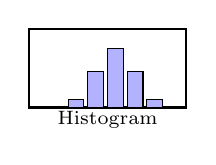
\begin{tikzpicture}[scale=0.5]
\draw[thick] (0,0) rectangle (4,2);
\foreach \x in {0.5,1,1.5,2,2.5,3,3.5} {
  \pgfmathsetmacro{\height}{1.5*exp(-2*(\x-2)*(\x-2))}
  \draw[fill=blue!30] (\x,0) rectangle (\x+0.4,\height);
}
\node at (2,-0.3) {\scriptsize Histogram};
\end{tikzpicture}

% Box Plot
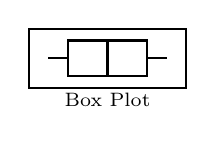
\begin{tikzpicture}[scale=0.5]
\draw[thick] (0,0) rectangle (4,1.5);
\draw[thick] (1,0.3) rectangle (3,1.2);
\draw[thick] (2,0.3) -- (2,1.2);
\draw[thick] (0.5,0.75) -- (1,0.75);
\draw[thick] (3,0.75) -- (3.5,0.75);
\node at (2,-0.3) {\scriptsize Box Plot};
\end{tikzpicture}

\vspace{0.3cm}
\textbf{Bivariate Visualizations:}
\vspace{0.2cm}

% Scatter Plot
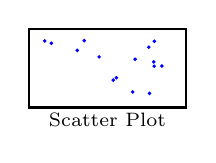
\begin{tikzpicture}[scale=0.5]
\draw[thick] (0,0) rectangle (4,2);
\foreach \i in {1,...,15} {
  \pgfmathsetmacro{\x}{0.3+3.4*rnd}
  \pgfmathsetmacro{\y}{0.3+1.4*rnd}
  \fill[blue] (\x,\y) circle (0.05);
}
\node at (2,-0.3) {\scriptsize Scatter Plot};
\end{tikzpicture}

% Correlation Heatmap

\begin{tikzpicture}[scale=0.4]
\foreach \i in {0,1,2,3} {
  \foreach \j in {0,1,2,3} {
    \pgfmathsetmacro{\color}{20+60*rnd}
    \fill[red!\color] (\i,\j) rectangle (\i+0.9,\j+0.9);
  }
}
\node at (2,-0.5) {\scriptsize Correlation Heatmap};
\end{tikzpicture}
\end{column}

\begin{column}{0.48\textwidth}
\textbf{Multivariate Visualizations:}
\vspace{0.2cm}

% Pair Plot
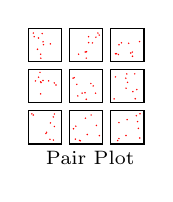
\begin{tikzpicture}[scale=0.35]
\foreach \i in {0,1,2} {
  \foreach \j in {0,1,2} {
    \draw (\i*1.5,\j*1.5) rectangle (\i*1.5+1.2,\j*1.5+1.2);
    \if \i=\j
      \foreach \k in {1,...,8} {
        \pgfmathsetmacro{\height}{0.8*exp(-2*(\k-4.5)*(\k-4.5)/4)}
        \draw[fill=blue!30] (\i*1.5+0.1*\k,\j*1.5) rectangle (\i*1.5+0.1*\k+0.08,\j*1.5+\height);
      }
    \else
      \foreach \k in {1,...,10} {
        \pgfmathsetmacro{\x}{\i*1.5+0.1+1.0*rnd}
        \pgfmathsetmacro{\y}{\j*1.5+0.1+1.0*rnd}
        \fill[red] (\x,\y) circle (0.03);
      }
    \fi
  }
}
\node at (2.25,-0.5) {\scriptsize Pair Plot};
\end{tikzpicture}

\vspace{0.3cm}
\textbf{Time Series:}
\vspace{0.2cm}

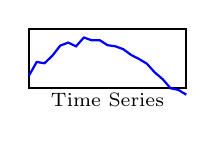
\begin{tikzpicture}[scale=0.5]
\draw[thick] (0,0) rectangle (4,1.5);
\draw[thick, blue] (0,0.3) \foreach \x in {0.2,0.4,...,4} {
  -- (\x,{0.3+0.8*sin(\x*180/3.14159)+0.2*rnd})
};
\node at (2,-0.3) {\scriptsize Time Series};
\end{tikzpicture}

\vspace{0.3cm}
\begin{exampleblock}{Python Code Examples}
\scriptsize
\texttt{sns.histplot(df['age'])} \\
\texttt{sns.scatterplot(x='age', y='salary', data=df)} \\
\texttt{sns.pairplot(df)} \\
\texttt{sns.heatmap(df.corr(), annot=True)}
\end{exampleblock}
\end{column}
\end{columns}
\end{frame}

\begin{frame}{Feature Selection: Choosing the Right Variables}
\begin{columns}[t]
\begin{column}{0.48\textwidth}
\textbf{Why Feature Selection?}
\begin{itemize}
\setlength{\itemsep}{1pt}
\item \textcolor{red}{\textbf{Curse of dimensionality}} - Too many features
\item \textcolor{blue}{\textbf{Overfitting}} - Model memorizes noise
\item \textcolor{green}{\textbf{Training time}} - Computational efficiency
\item \textcolor{orange}{\textbf{Interpretability}} - Simpler models
\end{itemize}

\vspace{0.3cm}
\textbf{Selection Methods:}
\begin{itemize}
\setlength{\itemsep}{1pt}
\item \textbf{Filter Methods:} Statistical tests, correlation
\item \textbf{Wrapper Methods:} Forward/backward selection
\item \textbf{Embedded Methods:} LASSO, Random Forest importance
\end{itemize}

\vspace{0.3cm}
\begin{block}{Correlation-based Selection}
\scriptsize
\texttt{corr\_matrix = df.corr().abs()} \\
\texttt{to\_drop = [col for col in upper\_tri.columns} \\
\texttt{\\phantom{\\ldots\\ldots\\ldots\\ldots}if any(upper\_tri[col] > 0.95)]}
\end{block}
\end{column}

\begin{column}{0.48\textwidth}
\textbf{Feature Importance Visualization:}
\vspace{0.2cm}

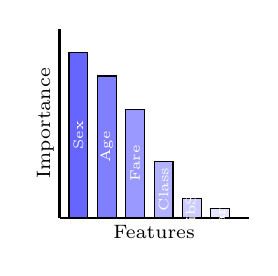
\begin{tikzpicture}[scale=0.6]
% Feature importance bar chart
\draw[thick] (0,0) -- (0,4);
\draw[thick] (0,0) -- (4,0);

% Bars with different heights
\draw[fill=blue!60] (0.2,0) rectangle (0.6,3.5) node[midway, rotate=90, white] {\tiny Sex};
\draw[fill=blue!50] (0.8,0) rectangle (1.2,3.0) node[midway, rotate=90, white] {\tiny Age};
\draw[fill=blue!40] (1.4,0) rectangle (1.8,2.3) node[midway, rotate=90, white] {\tiny Fare};
\draw[fill=blue!30] (2.0,0) rectangle (2.4,1.2) node[midway, rotate=90, white] {\tiny Class};
\draw[fill=blue!20] (2.6,0) rectangle (3.0,0.4) node[midway, rotate=90, white] {\tiny SibSp};
\draw[fill=blue!10] (3.2,0) rectangle (3.6,0.2) node[midway, rotate=90, white] {\tiny Parch};

\node[rotate=90] at (-0.3,2) {\scriptsize Importance};
\node at (2,-0.3) {\scriptsize Features};
\end{tikzpicture}

\vspace{0.3cm}
\begin{exampleblock}{Sklearn Feature Selection}
\scriptsize
\texttt{from sklearn.feature\_selection import SelectKBest}\\
\texttt{selector = SelectKBest(f\_classif, k=5)}\\
\texttt{X\_selected = selector.fit\_transform(X, y)}\\
\vspace{0.1cm}
\texttt{rf = RandomForestClassifier()}\\
\texttt{importances = rf.feature\_importances\_}
\end{exampleblock}
\end{column}
\end{columns}
\end{frame}

\begin{frame}{Correlation and Advanced Relationships}
\begin{columns}[t]
\begin{column}{0.48\textwidth}
\textbf{Correlation Types:}
\begin{itemize}
\setlength{\itemsep}{1pt}
\item \textbf{Pearson:} Linear relationships (continuous)
\item \textbf{Spearman:} Monotonic relationships (ordinal)
\item \textbf{Kendall:} Rank-based, robust to outliers
\end{itemize}

\vspace{0.3cm}
\begin{block}{Interpretation}
\begin{itemize}
\setlength{\itemsep}{1pt}
\item $|r| < 0.3$: Weak
\item $0.3 \leq |r| < 0.7$: Moderate
\item $|r| \geq 0.7$: Strong
\item $r = 0$: No linear correlation
\end{itemize}
\end{block}

\textbf{Multicollinearity:}
\begin{itemize}
\setlength{\itemsep}{1pt}
\item \textbf{VIF:} Variance Inflation Factor
\item \textbf{Condition Index:} Eigenvalue analysis
\item \textbf{Tolerance:} $1 - R^2$ from regression
\end{itemize}
\end{column}

\begin{column}{0.48\textwidth}
\textbf{Visualization Techniques:}
\begin{itemize}
\setlength{\itemsep}{1pt}
\item \textcolor{blue}{Heatmaps:} Correlation matrices
\item \textcolor{red}{Scatter plots:} Pairwise relationships
\item \textcolor{green}{Pair plots:} Multiple variables
\item \textcolor{purple}{Parallel coordinates:} High-dimensional
\end{itemize}

\vspace{0.3cm}
\begin{block}{Advanced Analysis}
\textbf{Categorical-Numerical:}
\begin{itemize}
\setlength{\itemsep}{1pt}
\item ANOVA F-test
\item Kruskal-Wallis test
\item Box plots by category
\end{itemize}

\textbf{Categorical-Categorical:}
\begin{itemize}
\setlength{\itemsep}{1pt}
\item Chi-square test
\item Cramér's V
\item Contingency tables
\end{itemize}
\end{block}
\end{column}
\end{columns}
\end{frame}

\begin{frame}{Feature Selection Example: Titanic Dataset}
\begin{columns}[t]
\begin{column}{0.48\textwidth}
\textbf{Available Features:}
\begin{itemize}
\setlength{\itemsep}{1pt}
\item \texttt{Pclass} - Passenger class (1,2,3)
\item \texttt{Sex} - Gender (male/female)
\item \texttt{Age} - Age in years
\item \texttt{SibSp} - Siblings/spouses aboard
\item \texttt{Parch} - Parents/children aboard
\item \texttt{Fare} - Ticket fare
\item \texttt{Embarked} - Port of embarkation
\item \texttt{Name} - Passenger name
\item \texttt{Ticket} - Ticket number
\item \texttt{Cabin} - Cabin number
\end{itemize}

\vspace{0.3cm}
\begin{block}{Feature Importance (Random Forest)}
\scriptsize
\begin{tabular}{|l|c|}
\hline
\textbf{Feature} & \textbf{Importance} \\
\hline
Sex & 0.31 \\
Age & 0.28 \\
Fare & 0.23 \\
Pclass & 0.12 \\
SibSp & 0.04 \\
Parch & 0.02 \\
\hline
\end{tabular}
\end{block}
\end{column}

\begin{column}{0.48\textwidth}
\textbf{Selection Strategy:}
\vspace{0.2cm}

\begin{alertblock}{Remove}
\begin{itemize}
\setlength{\itemsep}{1pt}
\item \textcolor{red}{\texttt{Name}} - High cardinality, no pattern
\item \textcolor{red}{\texttt{Ticket}} - Unique identifiers
\item \textcolor{red}{\texttt{Cabin}} - 77\% missing
\end{itemize}
\end{alertblock}

\begin{block}{Engineer}
\begin{itemize}
\setlength{\itemsep}{1pt}
\item \textcolor{blue}{\texttt{Title}} - Extract from Name (Mr, Mrs, Dr)
\item \textcolor{blue}{\texttt{FamilySize}} - SibSp + Parch + 1
\item \textcolor{blue}{\texttt{IsAlone}} - FamilySize == 1
\item \textcolor{blue}{\texttt{AgeBin}} - Bin Age into groups
\end{itemize}
\end{block}

\textbf{Final Feature Set:}
\begin{itemize}
\setlength{\itemsep}{1pt}
\item \textcolor{green}{Pclass, Sex, Age, Fare}
\item \textcolor{green}{Embarked, Title, FamilySize, IsAlone}
\end{itemize}

\vspace{0.2cm}
\textbf{Performance Impact:}
\scriptsize
\begin{tabular}{|l|c|}
\hline
\textbf{Feature Set} & \textbf{Accuracy} \\
\hline
All original & 0.79 \\
Selected + Engineered & 0.83 \\
\hline
\end{tabular}
\end{column}
\end{columns}
\end{frame}

\begin{frame}{Complete ML Pipeline: From Raw Data to Model}
\begin{columns}[t]
\begin{column}{0.48\textwidth}
\textbf{Pipeline Stages:}
\vspace{0.2cm}

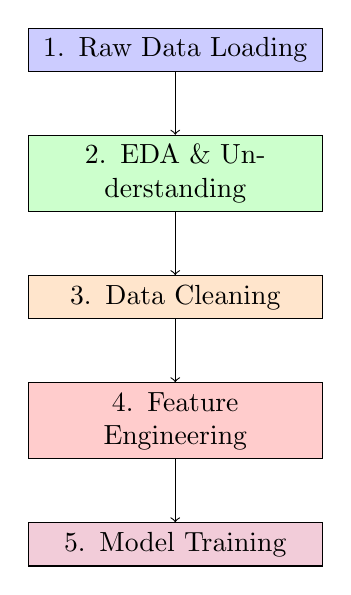
\begin{tikzpicture}[node distance=0.8cm]
\node[rectangle, draw, fill=blue!20, text width=3.5cm, text centered] (raw) {1. Raw Data Loading};
\node[rectangle, draw, fill=green!20, text width=3.5cm, text centered, below=of raw] (eda) {2. EDA \& Understanding};
\node[rectangle, draw, fill=orange!20, text width=3.5cm, text centered, below=of eda] (clean) {3. Data Cleaning};
\node[rectangle, draw, fill=red!20, text width=3.5cm, text centered, below=of clean] (feature) {4. Feature Engineering};
\node[rectangle, draw, fill=purple!20, text width=3.5cm, text centered, below=of feature] (model) {5. Model Training};

\draw[->] (raw) -- (eda);
\draw[->] (eda) -- (clean);
\draw[->] (clean) -- (feature);
\draw[->] (feature) -- (model);
\end{tikzpicture}
\end{column}

\begin{column}{0.48\textwidth}
\begin{exampleblock}{Sample Pipeline Code}
\scriptsize
\texttt{pipeline = Pipeline([} \\
\texttt{\\phantom{\\ldots}('scaler', StandardScaler()),} \\
\texttt{\\phantom{\\ldots}('classifier', RandomForestClassifier())}\\texttt{])} \\
\texttt{pipeline.fit(X\_train, y\_train)} \\
\texttt{accuracy = pipeline.score(X\_test, y\_test)}
\end{exampleblock}

\vspace{0.3cm}
\textbf{Key Benefits:}
\begin{itemize}
\setlength{\itemsep}{1pt}
\item \textcolor{blue}{Reproducible} experiments
\item \textcolor{red}{Prevents} data leakage
\item \textcolor{green}{Easy} hyperparameter tuning
\item \textcolor{orange}{Simplified} deployment
\end{itemize}
\end{column}
\end{columns}
\end{frame}

\begin{frame}{Visualization Best Practices}
\begin{columns}[t]
\begin{column}{0.48\textwidth}
\textbf{Chart Selection Guide:}
\begin{itemize}
\setlength{\itemsep}{1pt}
\item \textbf{Distribution:} Histogram, KDE, box plot
\item \textbf{Comparison:} Bar chart, grouped bar
\item \textbf{Relationship:} Scatter plot, line plot
\item \textbf{Composition:} Stacked bar, pie (avoid)
\item \textbf{Trend:} Line plot, area chart
\end{itemize}

\vspace{0.3cm}
\begin{block}{Design Principles}
\begin{itemize}
\setlength{\itemsep}{1pt}
\item \textcolor{red}{Clarity:} Simple, uncluttered
\item \textcolor{blue}{Accuracy:} Proper scaling, no misleading
\item \textcolor{green}{Efficiency:} Maximize data-ink ratio
\item \textcolor{orange}{Aesthetics:} Professional appearance
\end{itemize}
\end{block}
\end{column}

\begin{column}{0.48\textwidth}
\textbf{Common Pitfalls:}
\begin{itemize}
\setlength{\itemsep}{1pt}
\item \textcolor{red}{$\times$} Truncated y-axes
\item \textcolor{red}{$\times$} 3D charts without purpose
\item \textcolor{red}{$\times$} Too many colors/categories
\item \textcolor{red}{$\times$} Poor aspect ratios
\item \textcolor{red}{$\times$} Missing context/labels
\end{itemize}

\vspace{0.3cm}
\textbf{Python Libraries:}
\begin{itemize}
\setlength{\itemsep}{1pt}
\item \textbf{Matplotlib:} Low-level, flexible
\item \textbf{Seaborn:} Statistical plots, attractive defaults
\item \textbf{Plotly:} Interactive, web-ready
\item \textbf{Bokeh:} Interactive, large datasets
\item \textbf{Altair:} Grammar of graphics
\end{itemize}

\textbf{Key Functions:}
\begin{itemize}
\setlength{\itemsep}{1pt}
\item \texttt{sns.pairplot()}, \texttt{sns.heatmap()}
\item \texttt{plt.subplots()}, \texttt{plt.hist()}
\item \texttt{df.plot()}, \texttt{df.hist()}
\end{itemize}
\end{column}
\end{columns}
\end{frame}

\begin{frame}{EDA Workflow and Tools}
\begin{columns}[t]
\begin{column}{0.48\textwidth}
\textbf{Systematic EDA Process:}
\begin{enumerate}
\setlength{\itemsep}{1pt}
\item \textbf{Initial Assessment}
   \begin{itemize}
   \item \texttt{df.shape}, \texttt{df.info()}
   \item \texttt{df.describe()}
   \item \texttt{df.head()}, \texttt{df.tail()}
   \end{itemize}
\item \textbf{Data Quality Check}
   \begin{itemize}
   \item Missing values analysis
   \item Duplicate detection
   \item Data type validation
   \end{itemize}
\item \textbf{Univariate Analysis}
   \begin{itemize}
   \item Distributions, outliers
   \item Summary statistics
   \end{itemize}
\item \textbf{Bivariate/Multivariate}
   \begin{itemize}
   \item Correlations, relationships
   \item Feature interactions
   \end{itemize}
\end{enumerate}
\end{column}

\begin{column}{0.48\textwidth}
\textbf{Automated EDA Tools:}
\begin{itemize}
\setlength{\itemsep}{1pt}
\item \textbf{Pandas Profiling:} Comprehensive reports
\item \textbf{AutoViz:} Automatic visualization
\item \textbf{SweetViz:} Interactive HTML reports
\item \textbf{DataPrep:} Fast EDA with minimal code
\end{itemize}

\vspace{0.3cm}
\begin{block}{Key Metrics to Track}
\begin{itemize}
\setlength{\itemsep}{1pt}
\item \textbf{Completeness:} \% non-missing values
\item \textbf{Uniqueness:} Duplicate rate
\item \textbf{Validity:} Data type consistency
\item \textbf{Distribution:} Skewness, normality
\item \textbf{Outliers:} Percentage beyond thresholds
\end{itemize}
\end{block}

\textbf{Documentation:}
\begin{itemize}
\setlength{\itemsep}{1pt}
\item Data dictionary
\item Assumptions and decisions
\item Transformation rationale
\item Quality issues found
\end{itemize}
\end{column}
\end{columns}
\end{frame}

\begin{frame}{Summary and Next Steps}
\begin{columns}[t]
\begin{column}{0.48\textwidth}
\textbf{EDA Deliverables:}
\begin{itemize}
\setlength{\itemsep}{1pt}
\item \textcolor{blue}{\textbf{Data Profile:}} Shape, types, quality
\item \textcolor{red}{\textbf{Quality Report:}} Missing, outliers, issues
\item \textcolor{green}{\textbf{Statistical Summary:}} Distributions, correlations
\item \textcolor{orange}{\textbf{Visualizations:}} Key patterns and relationships
\item \textcolor{purple}{\textbf{Insights:}} Business-relevant findings
\end{itemize}

\vspace{0.3cm}
\begin{block}{Critical Questions Answered}
\begin{itemize}
\setlength{\itemsep}{1pt}
\item What is the data quality?
\item What patterns exist?
\item Which features are important?
\item What preprocessing is needed?
\item Are there data collection issues?
\end{itemize}
\end{block}
\end{column}

\begin{column}{0.48\textwidth}
\textbf{Post-EDA Actions:}
\begin{enumerate}
\setlength{\itemsep}{1pt}
\item \textbf{Data Cleaning}
   \begin{itemize}
   \item Handle missing values
   \item Remove/treat outliers
   \item Fix data quality issues
   \end{itemize}
\item \textbf{Feature Engineering}
   \begin{itemize}
   \item Create new features
   \item Transform distributions
   \item Encode categorical variables
   \end{itemize}
\item \textbf{Feature Selection}
   \begin{itemize}
   \item Remove redundant features
   \item Select informative variables
   \item Address multicollinearity
   \end{itemize}
\item \textbf{Model Preparation}
   \begin{itemize}
   \item Split data
   \item Scale/normalize
   \item Validation strategy
   \end{itemize}
\end{enumerate}

\textbf{Remember:} EDA is iterative and informs all subsequent ML pipeline decisions.
\end{column}
\end{columns}
\end{frame}

\end{document}